% Graphic for TeX using PGF
% Title: /Users/frankrosner/Documents/Uni/MasterThesis/writeup/img/apm_vectors.dia
% Creator: Dia v0.97.2
% CreationDate: Fri Jul 25 14:23:14 2014
% For: frankrosner
% \usepackage{tikz}
% The following commands are not supported in PSTricks at present
% We define them conditionally, so when they are implemented,
% this pgf file will use them.
\ifx\du\undefined
  \newlength{\du}
\fi
\setlength{\du}{15\unitlength}
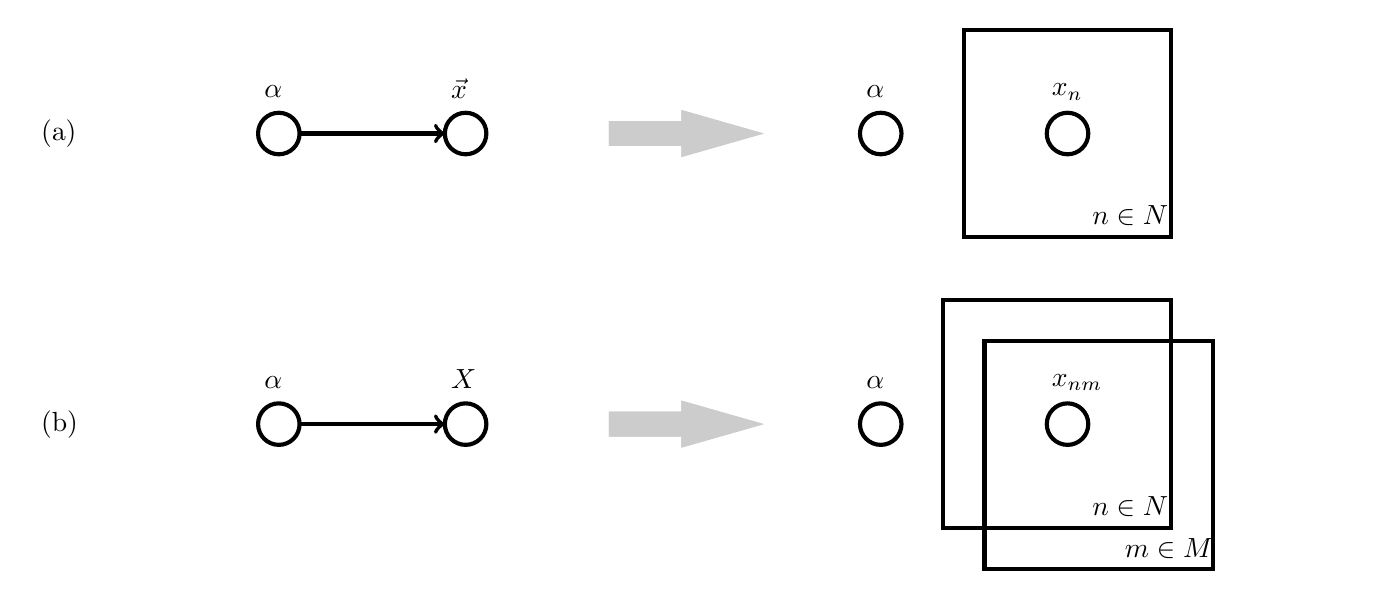
\begin{tikzpicture}
\pgftransformxscale{1.000000}
\pgftransformyscale{-1.000000}
\definecolor{dialinecolor}{rgb}{0.000000, 0.000000, 0.000000}
\pgfsetstrokecolor{dialinecolor}
\definecolor{dialinecolor}{rgb}{1.000000, 1.000000, 1.000000}
\pgfsetfillcolor{dialinecolor}
\pgfsetlinewidth{0.100000\du}
\pgfsetdash{}{0pt}
\pgfsetdash{}{0pt}
\pgfsetmiterjoin
\definecolor{dialinecolor}{rgb}{1.000000, 1.000000, 1.000000}
\pgfsetstrokecolor{dialinecolor}
\draw (6.000000\du,9.000000\du)--(6.000000\du,22.000000\du)--(38.000000\du,22.000000\du)--(38.000000\du,9.000000\du)--cycle;
\pgfsetlinewidth{0.100000\du}
\pgfsetdash{}{0pt}
\pgfsetdash{}{0pt}
\pgfsetmiterjoin
\definecolor{dialinecolor}{rgb}{0.000000, 0.000000, 0.000000}
\pgfsetstrokecolor{dialinecolor}
\draw (28.500000\du,9.000000\du)--(28.500000\du,14.000000\du)--(33.500000\du,14.000000\du)--(33.500000\du,9.000000\du)--cycle;
% setfont left to latex
\definecolor{dialinecolor}{rgb}{0.000000, 0.000000, 0.000000}
\pgfsetstrokecolor{dialinecolor}
\node[anchor=east] at (33.694600\du,13.483800\du){$n \in N$};
% setfont left to latex
\definecolor{dialinecolor}{rgb}{0.000000, 0.000000, 0.000000}
\pgfsetstrokecolor{dialinecolor}
\node[anchor=west] at (30.351400\du,10.500000\du){$x_n$};
\definecolor{dialinecolor}{rgb}{1.000000, 1.000000, 1.000000}
\pgfsetfillcolor{dialinecolor}
\pgfpathellipse{\pgfpoint{16.500000\du}{11.500000\du}}{\pgfpoint{0.500000\du}{0\du}}{\pgfpoint{0\du}{0.500000\du}}
\pgfusepath{fill}
\pgfsetlinewidth{0.100000\du}
\pgfsetdash{}{0pt}
\pgfsetdash{}{0pt}
\definecolor{dialinecolor}{rgb}{0.000000, 0.000000, 0.000000}
\pgfsetstrokecolor{dialinecolor}
\pgfpathellipse{\pgfpoint{16.500000\du}{11.500000\du}}{\pgfpoint{0.500000\du}{0\du}}{\pgfpoint{0\du}{0.500000\du}}
\pgfusepath{stroke}
% setfont left to latex
\definecolor{dialinecolor}{rgb}{0.000000, 0.000000, 0.000000}
\pgfsetstrokecolor{dialinecolor}
\node[anchor=west] at (15.881100\du,10.410800\du){$\vec x$};
\definecolor{dialinecolor}{rgb}{1.000000, 1.000000, 1.000000}
\pgfsetfillcolor{dialinecolor}
\pgfpathellipse{\pgfpoint{12.000000\du}{11.500000\du}}{\pgfpoint{0.500000\du}{0\du}}{\pgfpoint{0\du}{0.500000\du}}
\pgfusepath{fill}
\pgfsetlinewidth{0.100000\du}
\pgfsetdash{}{0pt}
\pgfsetdash{}{0pt}
\definecolor{dialinecolor}{rgb}{0.000000, 0.000000, 0.000000}
\pgfsetstrokecolor{dialinecolor}
\pgfpathellipse{\pgfpoint{12.000000\du}{11.500000\du}}{\pgfpoint{0.500000\du}{0\du}}{\pgfpoint{0\du}{0.500000\du}}
\pgfusepath{stroke}
% setfont left to latex
\definecolor{dialinecolor}{rgb}{0.000000, 0.000000, 0.000000}
\pgfsetstrokecolor{dialinecolor}
\node[anchor=west] at (11.381100\du,10.500000\du){$\alpha$};
\pgfsetlinewidth{0.100000\du}
\pgfsetdash{}{0pt}
\pgfsetdash{}{0pt}
\pgfsetbuttcap
{
\definecolor{dialinecolor}{rgb}{0.000000, 0.000000, 0.000000}
\pgfsetfillcolor{dialinecolor}
% was here!!!
\pgfsetarrowsend{to}
\definecolor{dialinecolor}{rgb}{0.000000, 0.000000, 0.000000}
\pgfsetstrokecolor{dialinecolor}
\draw (12.500000\du,11.500000\du)--(16.000000\du,11.500000\du);
}
\definecolor{dialinecolor}{rgb}{1.000000, 1.000000, 1.000000}
\pgfsetfillcolor{dialinecolor}
\pgfpathellipse{\pgfpoint{31.000000\du}{11.500000\du}}{\pgfpoint{0.500000\du}{0\du}}{\pgfpoint{0\du}{0.500000\du}}
\pgfusepath{fill}
\pgfsetlinewidth{0.100000\du}
\pgfsetdash{}{0pt}
\pgfsetdash{}{0pt}
\definecolor{dialinecolor}{rgb}{0.000000, 0.000000, 0.000000}
\pgfsetstrokecolor{dialinecolor}
\pgfpathellipse{\pgfpoint{31.000000\du}{11.500000\du}}{\pgfpoint{0.500000\du}{0\du}}{\pgfpoint{0\du}{0.500000\du}}
\pgfusepath{stroke}
\definecolor{dialinecolor}{rgb}{1.000000, 1.000000, 1.000000}
\pgfsetfillcolor{dialinecolor}
\pgfpathellipse{\pgfpoint{26.500000\du}{11.500000\du}}{\pgfpoint{0.500000\du}{0\du}}{\pgfpoint{0\du}{0.500000\du}}
\pgfusepath{fill}
\pgfsetlinewidth{0.100000\du}
\pgfsetdash{}{0pt}
\pgfsetdash{}{0pt}
\definecolor{dialinecolor}{rgb}{0.000000, 0.000000, 0.000000}
\pgfsetstrokecolor{dialinecolor}
\pgfpathellipse{\pgfpoint{26.500000\du}{11.500000\du}}{\pgfpoint{0.500000\du}{0\du}}{\pgfpoint{0\du}{0.500000\du}}
\pgfusepath{stroke}
% setfont left to latex
\definecolor{dialinecolor}{rgb}{0.000000, 0.000000, 0.000000}
\pgfsetstrokecolor{dialinecolor}
\node[anchor=west] at (25.881100\du,10.500000\du){$\alpha$};
\pgfsetlinewidth{0.100000\du}
\pgfsetdash{}{0pt}
\pgfsetdash{}{0pt}
\pgfsetbuttcap
\pgfsetmiterjoin
\pgfsetlinewidth{0.100000\du}
\pgfsetbuttcap
\pgfsetmiterjoin
\pgfsetdash{}{0pt}
\definecolor{dialinecolor}{rgb}{0.800000, 0.800000, 0.800000}
\pgfsetfillcolor{dialinecolor}
\fill (20.000000\du,11.250000\du)--(21.750000\du,11.250000\du)--(21.750000\du,11.000000\du)--(23.500000\du,11.500000\du)--(21.750000\du,12.000000\du)--(21.750000\du,11.750000\du)--(20.000000\du,11.750000\du)--cycle;
\definecolor{dialinecolor}{rgb}{0.800000, 0.800000, 0.800000}
\pgfsetstrokecolor{dialinecolor}
\draw (20.000000\du,11.250000\du)--(21.750000\du,11.250000\du)--(21.750000\du,11.000000\du)--(23.500000\du,11.500000\du)--(21.750000\du,12.000000\du)--(21.750000\du,11.750000\du)--(20.000000\du,11.750000\du)--cycle;
\pgfsetbuttcap
\pgfsetmiterjoin
\pgfsetdash{}{0pt}
\definecolor{dialinecolor}{rgb}{0.800000, 0.800000, 0.800000}
\pgfsetstrokecolor{dialinecolor}
\draw (20.000000\du,11.250000\du)--(21.750000\du,11.250000\du)--(21.750000\du,11.000000\du)--(23.500000\du,11.500000\du)--(21.750000\du,12.000000\du)--(21.750000\du,11.750000\du)--(20.000000\du,11.750000\du)--cycle;
\pgfsetlinewidth{0.100000\du}
\pgfsetdash{}{0pt}
\pgfsetdash{}{0pt}
\pgfsetmiterjoin
\definecolor{dialinecolor}{rgb}{0.000000, 0.000000, 0.000000}
\pgfsetstrokecolor{dialinecolor}
\draw (29.000000\du,16.500000\du)--(29.000000\du,22.000000\du)--(34.500000\du,22.000000\du)--(34.500000\du,16.500000\du)--cycle;
\pgfsetlinewidth{0.100000\du}
\pgfsetdash{}{0pt}
\pgfsetdash{}{0pt}
\pgfsetmiterjoin
\definecolor{dialinecolor}{rgb}{0.000000, 0.000000, 0.000000}
\pgfsetstrokecolor{dialinecolor}
\draw (28.000000\du,15.500000\du)--(28.000000\du,21.000000\du)--(33.500000\du,21.000000\du)--(33.500000\du,15.500000\du)--cycle;
% setfont left to latex
\definecolor{dialinecolor}{rgb}{0.000000, 0.000000, 0.000000}
\pgfsetstrokecolor{dialinecolor}
\node[anchor=east] at (33.694600\du,20.483800\du){$n \in N$};
% setfont left to latex
\definecolor{dialinecolor}{rgb}{0.000000, 0.000000, 0.000000}
\pgfsetstrokecolor{dialinecolor}
\node[anchor=west] at (30.351400\du,17.500000\du){$x_{nm}$};
\definecolor{dialinecolor}{rgb}{1.000000, 1.000000, 1.000000}
\pgfsetfillcolor{dialinecolor}
\pgfpathellipse{\pgfpoint{16.500000\du}{18.500000\du}}{\pgfpoint{0.500000\du}{0\du}}{\pgfpoint{0\du}{0.500000\du}}
\pgfusepath{fill}
\pgfsetlinewidth{0.100000\du}
\pgfsetdash{}{0pt}
\pgfsetdash{}{0pt}
\definecolor{dialinecolor}{rgb}{0.000000, 0.000000, 0.000000}
\pgfsetstrokecolor{dialinecolor}
\pgfpathellipse{\pgfpoint{16.500000\du}{18.500000\du}}{\pgfpoint{0.500000\du}{0\du}}{\pgfpoint{0\du}{0.500000\du}}
\pgfusepath{stroke}
% setfont left to latex
\definecolor{dialinecolor}{rgb}{0.000000, 0.000000, 0.000000}
\pgfsetstrokecolor{dialinecolor}
\node[anchor=west] at (15.881100\du,17.410800\du){$X$};
\definecolor{dialinecolor}{rgb}{1.000000, 1.000000, 1.000000}
\pgfsetfillcolor{dialinecolor}
\pgfpathellipse{\pgfpoint{12.000000\du}{18.500000\du}}{\pgfpoint{0.500000\du}{0\du}}{\pgfpoint{0\du}{0.500000\du}}
\pgfusepath{fill}
\pgfsetlinewidth{0.100000\du}
\pgfsetdash{}{0pt}
\pgfsetdash{}{0pt}
\definecolor{dialinecolor}{rgb}{0.000000, 0.000000, 0.000000}
\pgfsetstrokecolor{dialinecolor}
\pgfpathellipse{\pgfpoint{12.000000\du}{18.500000\du}}{\pgfpoint{0.500000\du}{0\du}}{\pgfpoint{0\du}{0.500000\du}}
\pgfusepath{stroke}
% setfont left to latex
\definecolor{dialinecolor}{rgb}{0.000000, 0.000000, 0.000000}
\pgfsetstrokecolor{dialinecolor}
\node[anchor=west] at (11.381100\du,17.500000\du){$\alpha$};
\pgfsetlinewidth{0.100000\du}
\pgfsetdash{}{0pt}
\pgfsetdash{}{0pt}
\pgfsetbuttcap
{
\definecolor{dialinecolor}{rgb}{0.000000, 0.000000, 0.000000}
\pgfsetfillcolor{dialinecolor}
% was here!!!
\pgfsetarrowsend{to}
\definecolor{dialinecolor}{rgb}{0.000000, 0.000000, 0.000000}
\pgfsetstrokecolor{dialinecolor}
\draw (12.500000\du,18.500000\du)--(16.000000\du,18.500000\du);
}
\definecolor{dialinecolor}{rgb}{1.000000, 1.000000, 1.000000}
\pgfsetfillcolor{dialinecolor}
\pgfpathellipse{\pgfpoint{31.000000\du}{18.500000\du}}{\pgfpoint{0.500000\du}{0\du}}{\pgfpoint{0\du}{0.500000\du}}
\pgfusepath{fill}
\pgfsetlinewidth{0.100000\du}
\pgfsetdash{}{0pt}
\pgfsetdash{}{0pt}
\definecolor{dialinecolor}{rgb}{0.000000, 0.000000, 0.000000}
\pgfsetstrokecolor{dialinecolor}
\pgfpathellipse{\pgfpoint{31.000000\du}{18.500000\du}}{\pgfpoint{0.500000\du}{0\du}}{\pgfpoint{0\du}{0.500000\du}}
\pgfusepath{stroke}
\definecolor{dialinecolor}{rgb}{1.000000, 1.000000, 1.000000}
\pgfsetfillcolor{dialinecolor}
\pgfpathellipse{\pgfpoint{26.500000\du}{18.500000\du}}{\pgfpoint{0.500000\du}{0\du}}{\pgfpoint{0\du}{0.500000\du}}
\pgfusepath{fill}
\pgfsetlinewidth{0.100000\du}
\pgfsetdash{}{0pt}
\pgfsetdash{}{0pt}
\definecolor{dialinecolor}{rgb}{0.000000, 0.000000, 0.000000}
\pgfsetstrokecolor{dialinecolor}
\pgfpathellipse{\pgfpoint{26.500000\du}{18.500000\du}}{\pgfpoint{0.500000\du}{0\du}}{\pgfpoint{0\du}{0.500000\du}}
\pgfusepath{stroke}
% setfont left to latex
\definecolor{dialinecolor}{rgb}{0.000000, 0.000000, 0.000000}
\pgfsetstrokecolor{dialinecolor}
\node[anchor=west] at (25.881100\du,17.500000\du){$\alpha$};
\pgfsetlinewidth{0.100000\du}
\pgfsetdash{}{0pt}
\pgfsetdash{}{0pt}
\pgfsetbuttcap
\pgfsetmiterjoin
\pgfsetlinewidth{0.100000\du}
\pgfsetbuttcap
\pgfsetmiterjoin
\pgfsetdash{}{0pt}
\definecolor{dialinecolor}{rgb}{0.800000, 0.800000, 0.800000}
\pgfsetfillcolor{dialinecolor}
\fill (20.000000\du,18.250000\du)--(21.750000\du,18.250000\du)--(21.750000\du,18.000000\du)--(23.500000\du,18.500000\du)--(21.750000\du,19.000000\du)--(21.750000\du,18.750000\du)--(20.000000\du,18.750000\du)--cycle;
\definecolor{dialinecolor}{rgb}{0.800000, 0.800000, 0.800000}
\pgfsetstrokecolor{dialinecolor}
\draw (20.000000\du,18.250000\du)--(21.750000\du,18.250000\du)--(21.750000\du,18.000000\du)--(23.500000\du,18.500000\du)--(21.750000\du,19.000000\du)--(21.750000\du,18.750000\du)--(20.000000\du,18.750000\du)--cycle;
\pgfsetbuttcap
\pgfsetmiterjoin
\pgfsetdash{}{0pt}
\definecolor{dialinecolor}{rgb}{0.800000, 0.800000, 0.800000}
\pgfsetstrokecolor{dialinecolor}
\draw (20.000000\du,18.250000\du)--(21.750000\du,18.250000\du)--(21.750000\du,18.000000\du)--(23.500000\du,18.500000\du)--(21.750000\du,19.000000\du)--(21.750000\du,18.750000\du)--(20.000000\du,18.750000\du)--cycle;
% setfont left to latex
\definecolor{dialinecolor}{rgb}{0.000000, 0.000000, 0.000000}
\pgfsetstrokecolor{dialinecolor}
\node[anchor=east] at (34.775000\du,21.500000\du){$m \in M$};
% setfont left to latex
\definecolor{dialinecolor}{rgb}{0.000000, 0.000000, 0.000000}
\pgfsetstrokecolor{dialinecolor}
\node[anchor=west] at (6.000000\du,11.500000\du){(a)};
% setfont left to latex
\definecolor{dialinecolor}{rgb}{0.000000, 0.000000, 0.000000}
\pgfsetstrokecolor{dialinecolor}
\node[anchor=west] at (6.000000\du,18.500000\du){(b)};
\end{tikzpicture}
